\documentclass[11pt]{exam}
\usepackage{geometry}                % See geometry.pdf to learn the layout options. There are lots.
\geometry{a4paper}                   % ... or a4paper or a5paper or ... 
%\geometry{landscape}                % Activate for for rotated page geometry
%\usepackage[parfill]{parskip}    % Activate to begin paragraphs with an empty line rather than an indent
\usepackage[french]{babel}
\usepackage[utf8x]{inputenc}
\usepackage[T1]{fontenc}

\usepackage[enseignants]{cave}
\usepackage{graphicx}
\usepackage{amssymb}
\usepackage{epstopdf}
\usepackage{listings}
\usepackage{url}
%\usepackage{framed}
\usepackage{verbatim}
\usepackage{fancyvrb,xcolor}

\DeclareGraphicsRule{.tif}{png}{.png}{`convert #1 `dirname #1`/`basename #1 .tif`.png}

\def\titrelong{Subsomption}
\def\titrecourt{Subsomption}
\def\revupar{SD}
\date{}                                           % Activate to display a given date or no date


\newsavebox{\FVerbBox}
\newenvironment{mycommand}
 {\VerbatimEnvironment
  \begin{center}
  \begin{lrbox}{\FVerbBox}
  \begin{minipage}{5.8in}
  \begin{Verbatim}}
 {\end{Verbatim}
  \end{minipage}
  \end{lrbox}
  \fcolorbox{blue!30}{gray!7}{\usebox{\FVerbBox}}
  \end{center}}


\begin{document}

Vous pourrez retrouver ce document à cette URL: \url{http://pages.isir.upmc.fr/~doncieux/public/IAR_2017/TME_IAR/}

L'objectif de ce TME est de doter un robot de comportements simples et d'étudier la complexité émergeant de la dynamique issue de l'interaction de ce robot et de ses règles de fonctionnement avec un environnement lui aussi très simple. Il consistera également une introduction à ROS par la pratique.

\section{Dans la salle de TME}

ROS ayant de nombreuses dépendances, il a été décidé, pour simplifier son installation, de passer par une machine virtuelle contenant une installation complète. Ce choix a limité la puissance disponible pour ROS, nous avons donc utilisé un simulateur très simple. Si vous avez accès à une machine puissante sur laquelle vous pouvez installer ROS, vous pourrez tester le même TME sur des robots plus sophistiqués, comme un turtlebot ou le PR2 en passant par le simulateur 3D Gazebo.


Pour lancer la machine virtuelle, dans le terminal, taper:
\begin{mycommand}
Vbox IAR_2017
\end{mycommand}
(puis entrez mot de passe)

~\\

{\huge ATTENTION: à partir de maintenant, toutes les commandes qui vous seront indiquées devront être lancées dans un terminal de la machine virtuelle.}

~\\

Pour avoir accès à internet, pensez à configurer le proxy de votre navigateur (dans la machine virtuelle): nom: proxy port: 3128 (à utiliser pour tous les protocoles).

\section{Préparation de l'environnement}

\textit{Les instructions suivantes expliquent comment installer les sources nécessaires au fonctionnement du TME. Ces opérations ont déjà été réalisées dans la machine virtuelle mise à votre disposition dans les salles de TME. Elles vous sont données pour que vous puissiez continuer hors des salles de TME si vous le souhaitez. Vous pouvez passer directement à la section suivante.}

Créer les répertoires \texttt{catkin\_ws/src}:
\begin{mycommand}
mkdir -p ~/catkin_ws/src
\end{mycommand}

Initialisez l'environnement catkin:
\begin{mycommand}
cd ~/catkin_ws/src
catkin_init_workspace
\end{mycommand}

\subsection{Récupération des sources et compilation}

Les codes sources utiles pour le TME sont téléchargeables à cette URL: \url{http://pages.isir.upmc.fr/~doncieux/public/IAR_2017/TME_IAR/}.

Vous aurez besoin de:
\begin{itemize}
\item \texttt{libfastsim.tar.gz}, la bibliothèque de simulation simple de robot. Vous pouvez aussi le récupérer avec \texttt{git}: \\ \texttt{git clone https://github.com/jbmouret/libfastsim}
\item \texttt{ros\_fastsim.tar.gz}, le noeud ROS permettant de s'interfacer avec cette bilbiothèque de simulation. Vous pouvez aussi le récupérer avec \texttt{git}: \\ \texttt{git clone https://github.com/jbmouret/ros\_fastsim}
\item \texttt{subsomption.tar.gz}: les noeuds que vous allez compléter pendant ce TME.
\end{itemize}

\subsection{Compilation des bibliothèques fournies}

\subsubsection{\texttt{libfastsim}}

Décompressez l'archive depuis la racine de votre compte et lancez les commandes suivantes dans le répertoire obtenu:
\begin{mycommand}
./waf configure
./waf
\end{mycommand}

\subsubsection{\texttt{ros\_fastsim}}

Allez dans le répertoire \texttt{catkin\_ws/src}, décompressez l'archive à partir de ce répertoire.
Depuis \texttt{catkin\_ws}, lancer les commandes:
\begin{mycommand}
source devel/setup.bash
catkin_make
\end{mycommand}

ATTENTION: vous devrez exécuter la première commande dans chaque nouveau terminal dans lequel vous voulez exécuter un noeud ROS.

\section{ROS}

\subsection{Guide de survie sous ROS}

ROS est un framework logiciel permettant de faciliter le développement d'applications robotiques. Il permet notamment d'échanger des messages entre des noeuds, de définir des services, etc. Il permet d'utiliser des noeuds développés pour un robot particulier sur un autre robot (du moins du point de vue informatique, rien ne garantit que le noeud marchera correctement avec le nouveau robot...). ROS permet aussi de passer très facilement du robot simulé au robot réel (là encore il est question de facilité "technique", mais ce n'est pas parce qu'un noeud peut facilement se connecter au robot réel qu'il marchera comme prévu...).

Chaque noeud de ROS est exécuté en parallèle des autres. Comme chaque noeud est susceptible de générer ses propres messages, il faut le lancer dans un terminal séparé. L'utilisation de ROS implique donc d'avoir de nombreux terminaux ouverts en même temps. Il est recommandé de les organiser, par exemple en ouvrant de nouveaux onglets plutôt que des fenêtres séparées.

\subsubsection{Préparation de l'environnement}

\subsubsection{ROSCORE}

ROS s'appuie sur un serveur qui est le chef d'orchestre et gèrera les échanges entre les différents noeuds, c'est \texttt{roscore}. Avant toute utilisation de ROS, il faut donc lancer ce serveur en tapant, dans un terminal la commande:
\begin{mycommand}
roscore
\end{mycommand}

Cette commande doit toujours être active pendant le TME.

\subsubsection{Lancement d'un noeud}

Le lancement d'un noeud ROS se fait avec la commande \texttt{rosrun}:
\begin{mycommand}
rosrun <package> <executable>
\end{mycommand}


Lorsqu'il faut lancer plusieurs noeuds en parallèle ou spécifier beaucoup d'arguments, il est possible de passer par la commande \texttt{roslaunch} qui prend en argument un fichier au format XML spécifiant les différents noeuds à lancer et la valeur des paramètres à utiliser. Nous présenterons plus loin comment l'utiliser.

\subsubsection{Topics}

Sous ROS un topic est un canal de communication entre des noeuds émetteurs et des noeuds récepteurs. Un topic est défini par un nom et un type de message.


Lister les topics disponibles:
\begin{mycommand}
rostopic list
\end{mycommand}

Afficher des détails sur un topic (type de message, émetteur(s), récepteur(s)):
\begin{mycommand}
rostopic info <nom de topic>
\end{mycommand}

Afficher les messages envoyés sur un topic:
\begin{mycommand}
rostopic echo <nom de topic>
\end{mycommand}

Pour avoir le descriptif d'un message:
\begin{mycommand}
rosmsg show <nom du message>
\end{mycommand}

\subsubsection{Autres}

Pour faire des tests avec un simulateur de tortue simple (pilotée par les flèches du clavier):
\begin{mycommand}
rosrun turtlesim turtlesim_node
rosrun turtlesim_turtle_teleop_key
\end{mycommand}


Pour voir le graphe des noeuds et des topics qui les relient:
\begin{mycommand}
rosrun rqt_graph rqt_graph
\end{mycommand}

Pour aller plus loin: \url {http://wiki.ros.org/}.

\section{Package \texttt{subsomption}}

Le package \texttt{subsomption} contient le squelette du code que vous aurez à compléter. Il contient également le fichier .launch à utiliser avec fastsim. Le noeud \texttt{ros\_fastsim} donne accès à un simulateur d'un robot circulaire, de type e-Puck, avec une gestion simplifiée de la physique et des collisions. 

Vous devrez d'abord décompresser l'archive \texttt{subsomption.tar.gz} dans le répertoire \\\texttt{~/catkin\_ws/src/}, puis exécuter les commandes:
\begin{mycommand}
cd ~/catkin_ws
catkin_make install
\end{mycommand}

Pour lancer fastsim sur l'environnement défini pour le TME, exécutez les commandes suivantes:

\begin{mycommand}
cd ~/catkin_ws/src/ros_fastsim/envs
roslaunch subsomption.launch
\end{mycommand}

Vous allez à présent créer votre architecture de subsomption. Elle s'appuiera sur le programme en python \texttt{subsomption\_architecture.py}. Ce noeud ROS, qui prend en argument le nombre $n$ de comportements à définir, écoute les topic \texttt{/subsomption/channel}\textit{i}, \textit{i} étant un entier compris entre $0$ et $n$. Sur ce topic sont envoyé des message selon le format suivant:
\begin{mycommand}
$ rosmsg show subsomption/channel
bool activated
float32 speed_left
float32 speed_right
\end{mycommand}

Le noeud de subsomption envoie à fastsim les commandes \texttt{speed\_left} et \texttt{speed\_right} venant du topic \texttt{/subsomption/channel}\textit{i} avec \textit{i} la valeur la plus haute pour laquelle \texttt{activated} vaut \texttt{True}.

~\\

\exercices

~\\

Vous devrez donc définir des comportements et les connecter aux différents canaux du noeud de subsomption. Le comportement actif qui sera connecté au canal d'indice le plus élevé sera celui qui aura la main sur le robot.

Le fichier \texttt{example.py} contient un exemple de noeud de comportement à remplir. Il vous est suggéré de partir de ce fichier pour créer vos propres comportements. Pour exécuter le comportement \texttt{comportement.py}, vous pouvez lancer:
\begin{mycommand}
rosrun subsomption comportement.py
\end{mycommand}
(\texttt{comportement.py} doit alors être exécutable), ou plus simplement:
\begin{mycommand}
python comportement.py
\end{mycommand}

Le noeud contenant l'architecture de sumbsomption devra tourner en parallèle:
\begin{mycommand}
python subsomption_architecture.py n
\end{mycommand}
où $n$ est le nombre de comportements souhaités.
 
~\\

L'évaluation se basera sur une démonstration de vos comportements. NE PARTEZ PAS DE LA SALLE DE TME SANS AVOIR FAIT CETTE DEMO. 

Vous devrez également envoyer un email à \url{stephane.doncieux@upmc.fr} avec, en attachement, les modules python que vous avez développés pour chaque question. Vous les accompagnerez de quelques commentaires expliquant vos choix.



~\\

{\Large Suivi de mur} 

\begin{questions}
\begin{quest}
Écrivez un premier comportement permettant au robot d'avancer tout droit et lancer son exécution sur le canal de priorité la plus faible.
\end{quest}
\begin{quest}
En cas de collision (détectée par les bumpers), écrivez un comportement permettant du robot de reculer et de faire demi-tour. Connectez-le au canal de priorité 2.
\end{quest}
\begin{quest}
Afin d'éviter les collisions, écrivez un comportement utilisant les lasers pour tourner avant de toucher un obstacle, vous lui donnerez la priorité 1. Vous pouvez changer la couverture des lasers en modifiant le fichier \texttt{envs/example.xml}.
\end{quest}
\begin{quest}
Définissez un ou plusieurs comportements permettant au robot de suivre les murs. Vous pourrez vous appuyer sur les comportements précédents ou en définir de nouveaux.
\end{quest}\end{questions}
 
~\\

{\Large Aspirateur} 

Vous allez maintenant programmer un robot aspirateur ROUMEBA pour qu'il se déplace aléatoirement dans une pièce, ceci dans le but de la nettoyer. 

\begin{figure}
\begin{center}
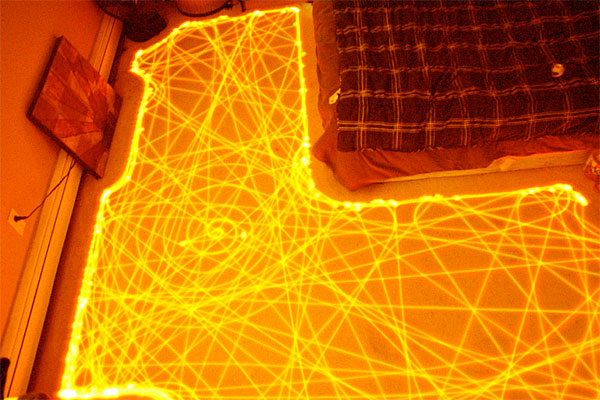
\includegraphics[width=0.7\linewidth]{./roomba-movements.jpg}
\end{center}
\caption{\label{fig:roomba} Trajectoire d'un robot aspirateur.}
\end{figure}

\begin{questions}
\begin{quest}
Définissez un ensemble de modules permettant de reproduire le comportement observé sur la figure \ref{fig:roomba}.
\end{quest}\end{questions}


~\\

{\Large Application sur le robot réel} 

Transférez vos comportements sur le robot réel. Les caractéristiques du laser sont les suivantes:
\begin{itemize}
\item angle\_min: -0.51
\item angle\_max: 0.49
\item angle\_inc: 0.00158
\item range\_min: 0.449
\item range\_max: 10. 
\end{itemize}


\end{document}  